% Number 420
% StaticEq
% Teeter totter
% MIT

% Watermark
\AddToShipoutPicture*{\BackgroundPic}

\addtocounter {ProbNum} {1}

\begin{floatingfigure}[r]{.35\textwidth}
\includegraphics[scale=.5]{/Users/jgates/desktop/latex/pics/staticeq1.png}
\end{floatingfigure}
 
{\bf \Large{\arabic{ProbNum}}} A long uniform board weighs 57.7 N (11.5 lbs) rests on a support at its mid point. Two children weighing 401.0 N (80.2 lbs) and 470.0 N (94.0 lbs) stand on the board so that the board is balanced. 

\bigskip
What is the upward force exerted on the board by the support? 

%\begin{center}
%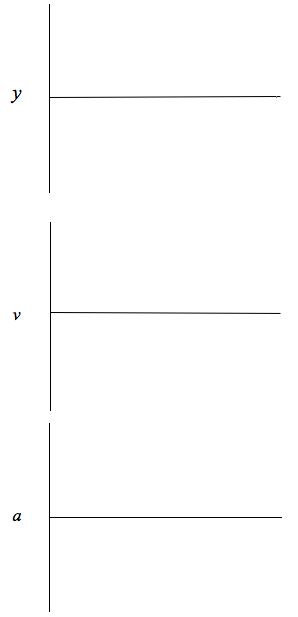
\includegraphics[scale=.85]{/Users/jgates/desktop/latex/pics/blankyvagraphstack.png}
%\end{center}


\vfill
\newpage